\chapter{System Architecture and Methodology}
\label{chap:architecture}

This chapter explains the pipeline from terrain data to estimated camera location. Each technique used is justified. Where a choice was made between alternatives, the reasoning is given.

\section{System Overview}
\label{sec:system_overview}

The system works in two stages.

\textbf{Preparation} (done once per study area):
\begin{enumerate}
    \item Download a digital elevation model (\Gls{dem}) for the target area.
    \item Ray-trace the terrain from many viewpoints to build a skyline database.
    \item Render synthetic mountain images from the same \Gls{dem} and train a sky-segmentation network.
\end{enumerate}

\textbf{On-device} (runs on the phone):
\begin{enumerate}
    \item Capture photographs with the phone camera.
    \item Segment the sky using the neural network.
    \item Convert the binary mask into a skyline profile.
    \item Match the profile against the database stored on the phone.
\end{enumerate}

\begin{figure}[H]
\centering

\includegraphics[width=0.85\textwidth]{src/images/pipeline_flow.pdf}
\caption{Pipeline overview.}
\label{fig:pipeline_flow}
\end{figure}

\section{Study Area}
\label{sec:study_area}

A 40\,km\,$\times$\,30\,km region in the Khumbu valley of eastern Nepal:

\begin{table}[H]
\centering
\caption{Study area bounds}
\label{tab:study_area}
\begin{tabular}{lc}
\toprule
\textbf{Corner} & \textbf{Coordinates} \\
\midrule
Northwest (NW) & 86.582$^\circ$E, 28.041$^\circ$N \\
Northeast (NE) & 86.989$^\circ$E, 28.041$^\circ$N \\
Southwest (SW) & 86.582$^\circ$E, 27.770$^\circ$N \\
Southeast (SE) & 86.989$^\circ$E, 27.770$^\circ$N \\
\bottomrule
\end{tabular}
\end{table}

Steep terrain, deep valleys, distinctive skylines. Trekking routes run through it, where \Gls{gnss} signals weaken behind ridges. The DEM is Copernicus GLO-30 (30\,m resolution).

\begin{figure}[H]
    \centering
    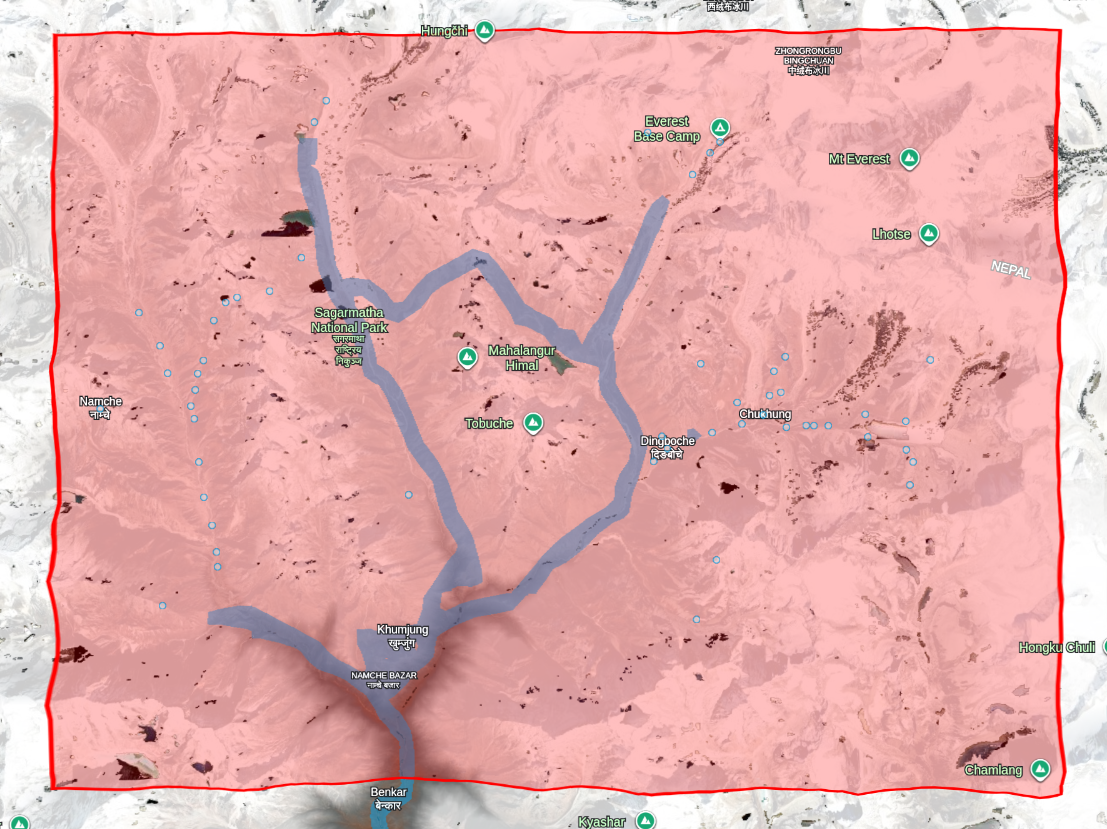
\includegraphics[width=0.7\textwidth]{src/images/roi.png}
    \caption{Study area.}
    \label{fig:study_area}
\end{figure}

\section{Reference Skyline Database}
\label{sec:db_gen}

Matching a photo against terrain data directly would require running ray-traces at query time, which is too slow for a phone. Precomputing the skyline from every viewpoint and storing it as a compact vector makes matching fast. The database stores what the skyline looks like from every point in the study area.

\subsection{Viewpoint Grid}

Candidate camera locations sit on a regular grid at 30\,m spacing. Every grid point gets a 360$^\circ$ horizon profile. The full set contains 1{,}338{,}650 viewpoints.

\begin{table}[H]
\centering
\caption{Database generation parameters}
\label{tab:db_params}
\begin{tabularx}{0.9\textwidth}{l X}
\toprule
\textbf{Parameter} & \textbf{Value} \\
\midrule
Grid spacing & 30\,m (matches DEM resolution) \\
Ray-trace distance & 30\,km in each direction \\
Azimuth bins & 720 (0.5$^\circ$ per bin, full 360$^\circ$) \\
Eye height & 1.6\,m above terrain \\
Total viewpoints & 1{,}338{,}650 \\
\bottomrule
\end{tabularx}
\end{table}

\subsection{Ray-Traced Horizon}

HORAYZON traces 720 rays per viewpoint through the DEM mesh up to 30\,km. For each direction $a$, the terrain elevation angle is

\begin{equation}
\theta_a = \tan^{-1}\!\left(\frac{h_t - h_o}{d_a}\right),
\label{eq:elevation_angle}
\end{equation}

\noindent where $h_t$ is the terrain elevation at the sample point, $h_o = h_{\mathrm{terrain}} + 1.6$\,m is the observer eye height, and $d_a$ is the horizontal distance. For each azimuth, only the maximum elevation angle along that ray is kept.

\subsection{Profile Filtering and Storage}

Flat or featureless profiles are removed: standard deviation below 1.5$^\circ$, or maximum elevation below 1.0$^\circ$. Surviving profiles are stored as integer vectors inside a compressed columnar file that supports reading small batches without loading the whole file. The compression reduces storage from roughly 0.96\,GB (raw \texttt{uint8}) to 486\,MB.

\section{Synthetic Training Data}
\label{sec:synthetic_data}

Training a segmentation network requires images with known sky-terrain boundaries. Synthetic rendering gives exact ground-truth masks for free.

\subsection{Compositing Process}

Three layers composited together:

\begin{enumerate}
    \item \textbf{Terrain mesh} --- DEM vertices textured with satellite imagery, rendered by PyRender (OpenGL-based, headless via EGL).
    \item \textbf{Sky backdrop} --- sky photos or gradients from one of six weather presets.
    \item \textbf{Camera effects} --- lens flare, rain streaks, sensor noise, vignette.
\end{enumerate}

\begin{figure}[H]
\centering

\includegraphics[width=0.82\textwidth]{src/images/synthetic_rendering.pdf}
\caption{Synthetic training data generation.}
\label{fig:synthetic_rendering}
\end{figure}

\subsection{Weather Presets}

Six presets: \textit{sunny}, \textit{overcast}, \textit{sunset}, \textit{stormy haze}, \textit{night}, \textit{rainy}. Each controls lighting, sky gradients, clouds, and fog. Random selection per sample prevents overfitting to one condition.

\section{Skyline Segmentation}
\label{sec:segmentation}

\subsection{U-Net Architecture}

A \Gls{unet} with MobileNetV3-Large encoder produces a per-pixel probability map from a $256 \times 256$ colour image. The encoder compresses the image into abstract features using depthwise separable convolutions, which factor a standard convolution into a depthwise step (one filter per channel) and a pointwise step ($1 \times 1$ convolution across channels). This reduces parameters while maintaining representational capacity. The decoder upsamples back through skip connections that copy fine spatial details from the encoder to the decoder at each resolution level. These skip connections are critical for preserving the sharp sky-terrain boundary.

\begin{figure}[H]
\centering
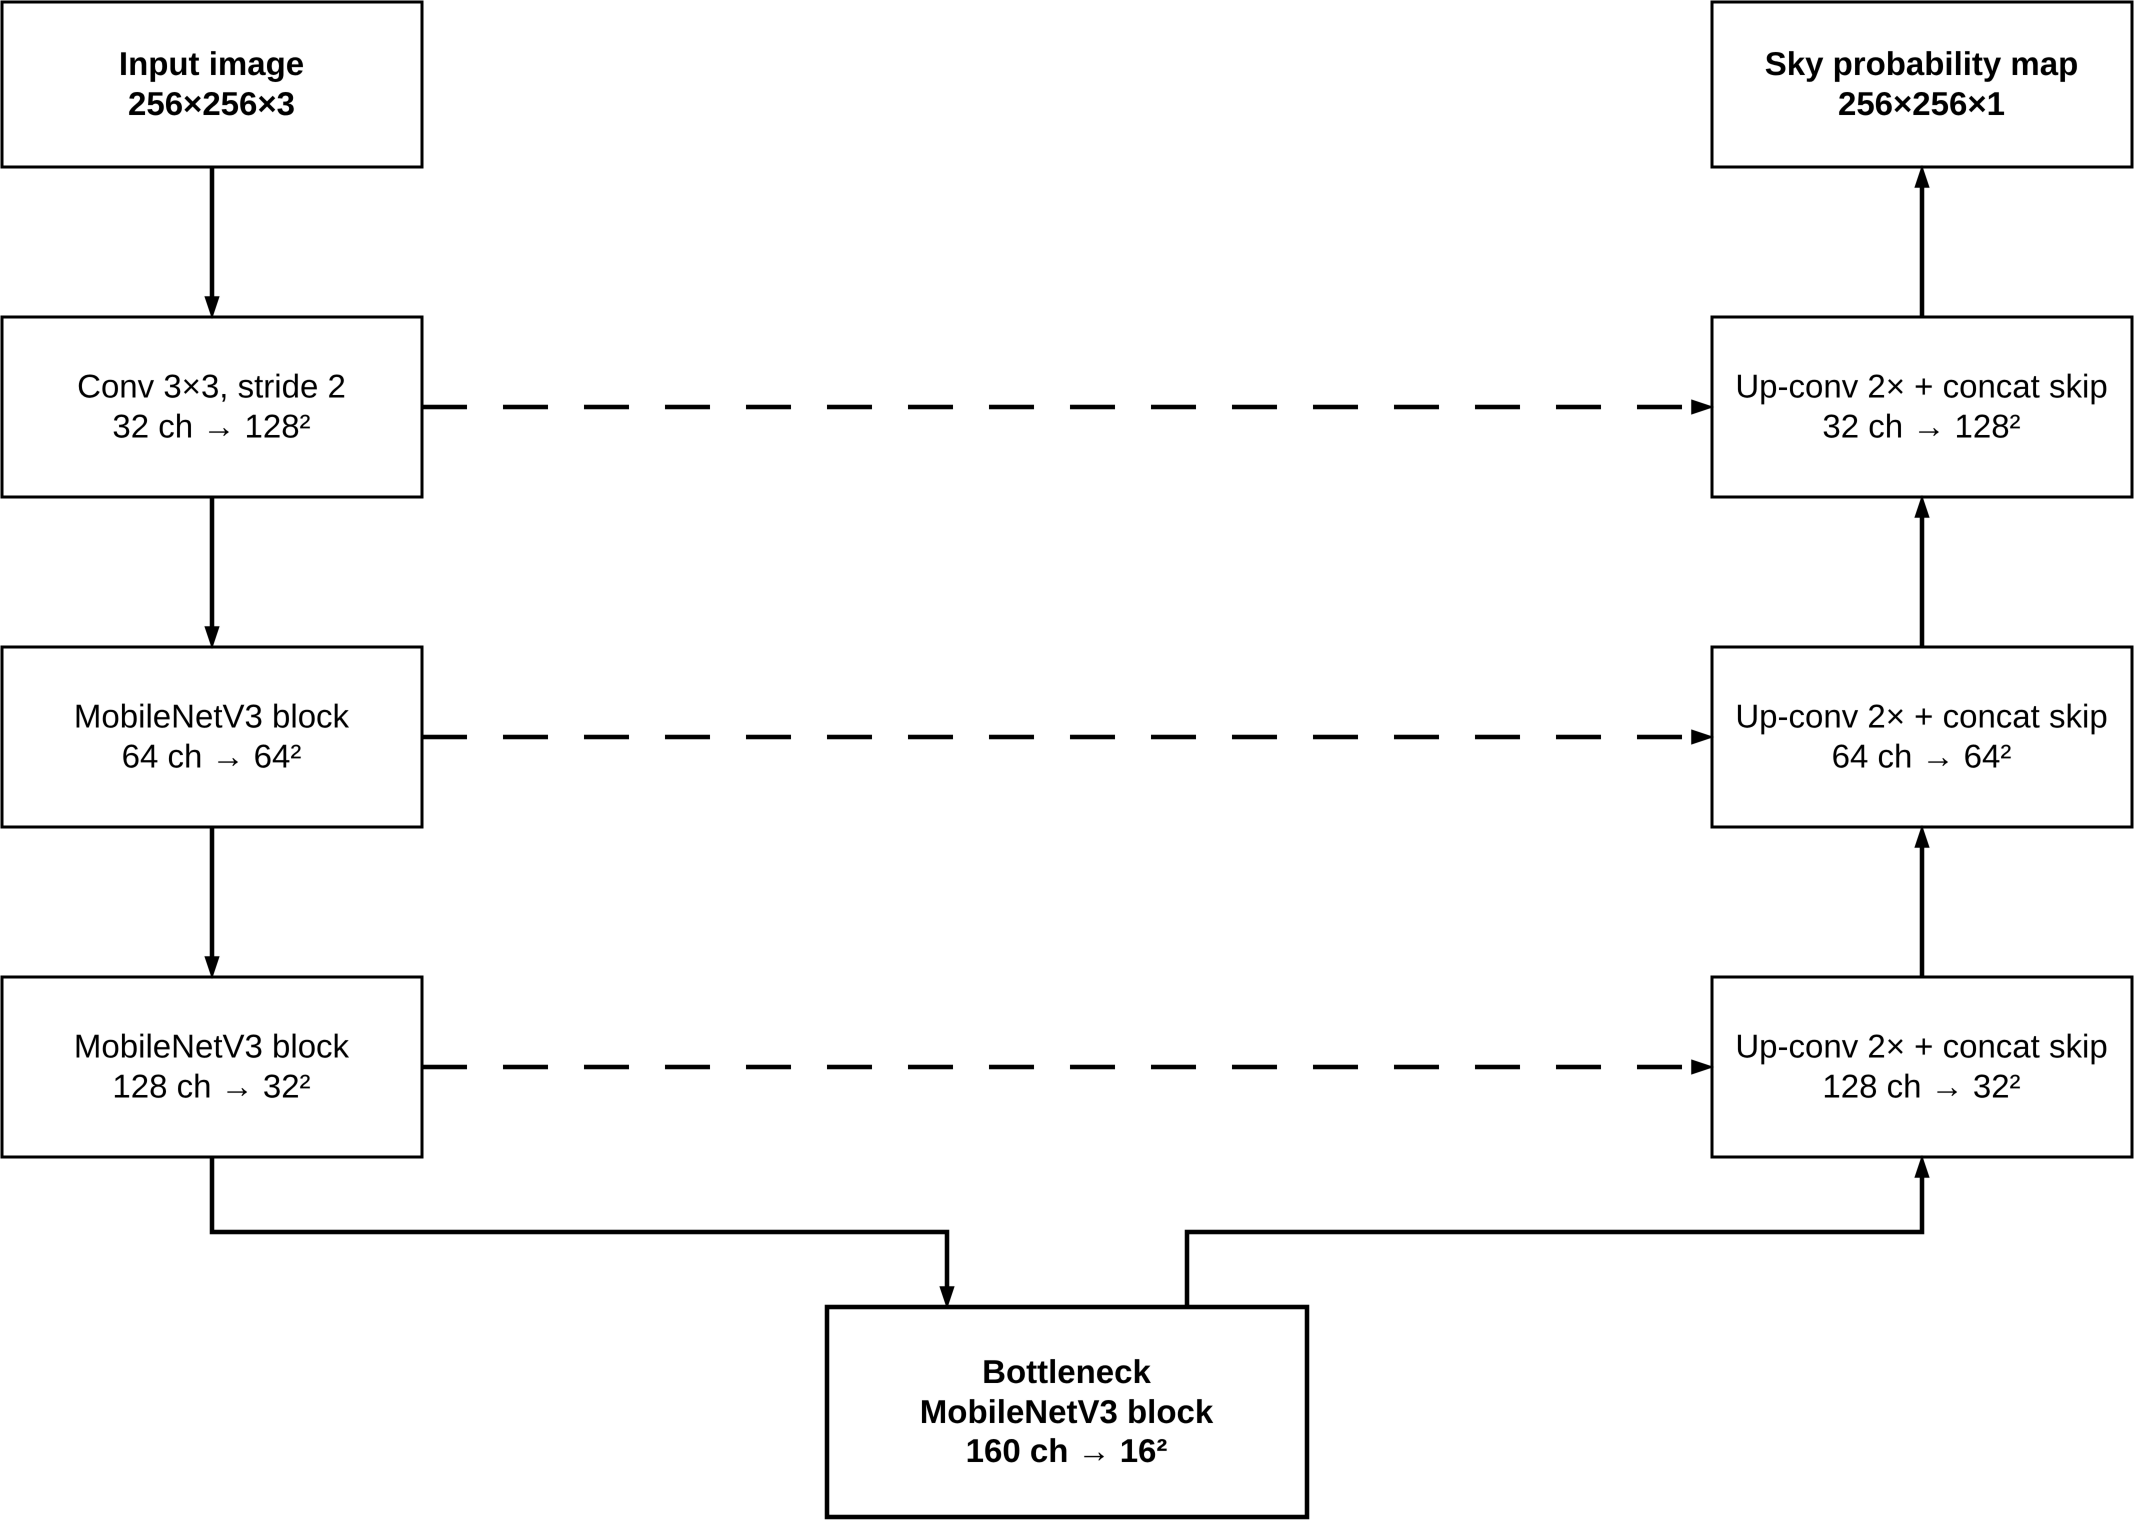
\includegraphics[width=0.88\textwidth]{src/images/figures/unet_architecture.png}
\caption{\Gls{unet} with MobileNetV3-Large encoder.}
\label{fig:unet_architecture}
\end{figure}

\subsection{Transfer Learning from ImageNet}

The encoder is pretrained on ImageNet, a large visual database containing roughly 14 million labelled photographs across 1000 categories. Although ImageNet contains no mountain images, its low-level features transfer well to mountain skylines. This works because early layers of convolutional networks learn universal visual primitives such as edges, textures, and colour gradients, which appear in any photographic domain. Using pretrained weights gives the network a strong starting point and reduces the amount of training data needed.

\subsection{Loss Function}

The network is trained with a combined loss of binary cross-entropy (\Gls{bce}) and soft Dice loss:

\begin{equation}
\mathcal{L} = \mathcal{L}_{\text{BCE}} + \mathcal{L}_{\text{Dice}},
\end{equation}

\noindent where
\begin{equation}
\mathcal{L}_{\text{BCE}} = -\frac{1}{N}\sum_{i=1}^{N}\Big[y_i \log \hat{p}_i + (1-y_i)\log(1-\hat{p}_i)\Big],
\end{equation}

\noindent $y_i$ is the ground-truth label (1 = sky, 0 = terrain), and $\hat{p}_i$ is the predicted probability for pixel $i$. The Dice loss is:

\begin{equation}
\mathcal{L}_{\text{Dice}} = 1 - \frac{2\sum_i y_i\hat{p}_i + \varepsilon}{\sum_i y_i + \sum_i \hat{p}_i + \varepsilon}, \qquad \varepsilon = 10^{-6}.
\end{equation}

BCE treats every pixel equally but is weak at boundaries. Dice focuses on overlap, giving more weight to the boundary where skyline accuracy matters. The combination addresses both problems.

\subsection{Training}

Trained on synthetic scenes and GeoPose3K. The optimizer is AdamW with cosine annealing. The best checkpoint is selected by validation \Gls{iou}.

\begin{table}[H]
\centering
\caption{Training parameters}
\label{tab:seg_training}
\begin{tabularx}{0.85\textwidth}{l X}
\toprule
\textbf{Parameter} & \textbf{Value} \\
\midrule
Architecture & \Gls{unet} + MobileNetV3-large \\
Pretraining & ImageNet (encoder weights) \\
Loss & \Gls{bce} + soft Dice \\
Optimizer & AdamW \\
Training data & GeoPose3K + synthetic scenes \\
\bottomrule
\end{tabularx}
\end{table}

\begin{figure}[H]
\centering
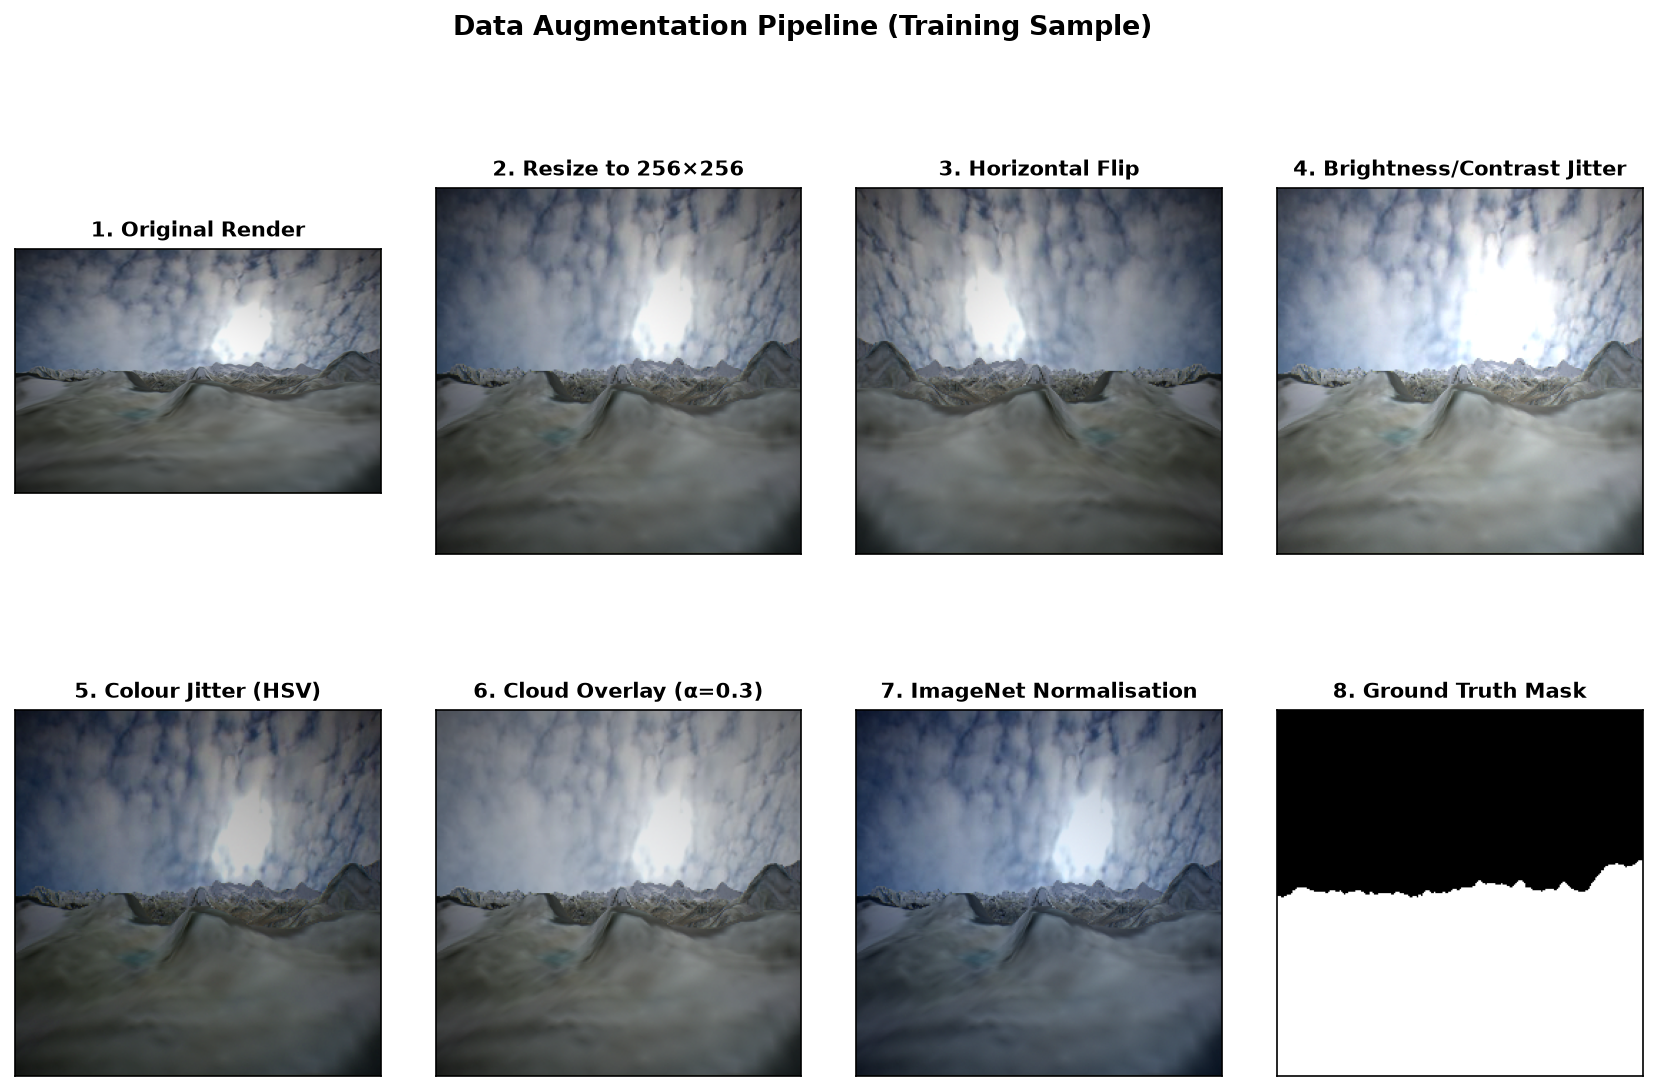
\includegraphics[width=0.92\textwidth]{src/images/fig_augmentation_pipeline.png}
\caption{Augmentation pipeline.}
\label{fig:augmentation_pipeline}
\end{figure}

\subsection{Post-Processing the Segmentation Mask}
\label{sec:post_processing}

The raw network output is a probability map. Several refinement steps clean up the boundary:

\paragraph{Thresholding.} Pixels with probability above 0.70 are classified as terrain, below as sky.

\paragraph{Top-connected filtering.} Connected components are computed on the sky mask. Only components that touch the top 15\% of the image are kept. This removes isolated sky blobs caused by reflections, shadows, or fog patches that the network incorrectly labelled as sky.

\paragraph{CLAHE dehazing.} Contrast-Limited Adaptive Histogram Equalisation is applied to the sky zone only. CLAHE divides the image into small tiles and equalises the histogram of each tile independently, limiting contrast amplification to avoid noise boost. This restores contrast in foggy or hazy regions where the sky-terrain boundary is washed out.

\paragraph{Multi-scale edge detection.} Canny edge detection runs at two scales: fine (Gaussian $\sigma = 3$, thresholds 30/150) and coarse ($\sigma = 7$, thresholds 20/100). The union of both edge maps captures boundaries at different sharpness levels. Edges are searched only within a narrow window ($\pm 10$ rows) around the U-Net boundary to avoid jumping to cloud edges far from the true terrain boundary.

\paragraph{Sub-pixel fitting.} For each column, the Sobel-Y gradient is computed near the detected boundary. A parabola is fitted to the three points surrounding the gradient peak:

\begin{equation}
\delta = \frac{g_{i+1} - g_{i-1}}{2(g_{i+1} - 2g_i + g_{i-1})},
\end{equation}

\noindent where $g_{i-1}$, $g_i$, $g_{i+1}$ are the gradient values at the peak and its neighbours. The sub-pixel offset $\delta$ is clamped to $[-0.5, 0.5]$. This reduces quantisation noise from integer row positions.

\paragraph{Outlier rejection and smoothing.} Boundary points more than 30\,px from the 5-neighbour median are rejected. The surviving boundary is interpolated across missing columns, then smoothed with a median filter ($k=9$) and a Gaussian filter ($\sigma = 7$, applied vertically). A two-pass slope constraint limits the boundary to at most 2\,px per column, removing sharp jumps from cloud edges.

\section{Skyline Extraction}
\label{sec:extraction}

The binary sky mask becomes a 1-D elevation-angle profile. Each column maps to an azimuth angle through the camera intrinsics. The first terrain pixel from the top marks the skyline. The result is interpolated onto a uniform grid matching the database. Phone cameras capture only 60$^\circ$--80$^\circ$ horizontal FOV, so the 1-D profile allows matching a partial view against the full 360$^\circ$ reference by sliding it around.

Profiles with standard deviation below 1.5$^\circ$, maximum elevation below 1.0$^\circ$, or boundary coverage below 50\% are rejected.

\section{Skyline Matching}
\label{sec:matching}

\subsection{Feature Representation}

Pearson normalised cross-correlation (\Gls{ncc}) measures profile similarity regardless of absolute elevation. Two z-scored channels are used: the elevation profile and its first derivative. Both weighted equally. The z-score normalisation ensures that profiles with different absolute elevation scales can be compared directly.

\subsection{Three-Stage Matching}

Scanning all 1.34M viewpoints at full resolution is too slow for a phone:

\begin{enumerate}
    \item \textbf{Coarse scan.} Sample every 12th viewpoint. \Gls{ncc} at every circular offset via \Gls{fft}. Top 5 kept.
    \item \textbf{Local refinement.} Expand to 12 neighbours per candidate, re-scored at full resolution. Top 30 advance.
    \item \textbf{FastDTW.} Re-rank top 30 using dynamic time warping \cite{salvador2007fastdtw}, which absorbs non-rigid shifts from camera tilt.
\end{enumerate}

\subsection{Three Scorers}

Different bandpass filters capture different terrain scales:

\begin{itemize}
    \item \textbf{Baseline} --- full elevation profile and its derivative.
    \item \textbf{Bandpass 1} --- ridge-scale features (2--8\,km). Created by subtracting a wide Gaussian from a narrow Gaussian in the frequency domain, isolating medium-scale terrain features.
    \item \textbf{Bandpass 2} --- valley-scale features (3--16\,km). Uses wider Gaussians to capture broad terrain patterns.
\end{itemize}

Reciprocal-Rank Fusion (RRF) combines all three ranked lists into one. RRF assigns each candidate a score of $\frac{1}{k + \text{rank}}$ for each scorer (with $k = 60$), then sums across scorers. Because RRF uses ranks, not raw scores, different scorer scales do not matter.

\subsection{Quality Filters}

Candidates with low correlation or small score gaps are rejected. The matcher returns \texttt{OK}, \texttt{LOW\_CONFIDENCE}, or \texttt{NO\_MATCH}.

\section{Mobile Client}
\label{sec:mobile}

Everything runs on the phone with no network needed. Device sensors (accelerometer and magnetometer) draw a level overlay on the camera preview. Two or three overlapping photos at different headings can be stitched into one wider horizon.

\begin{figure}[H]
\centering
\begin{adjustbox}{max totalsize={0.78\textwidth}{0.82\textheight},center}
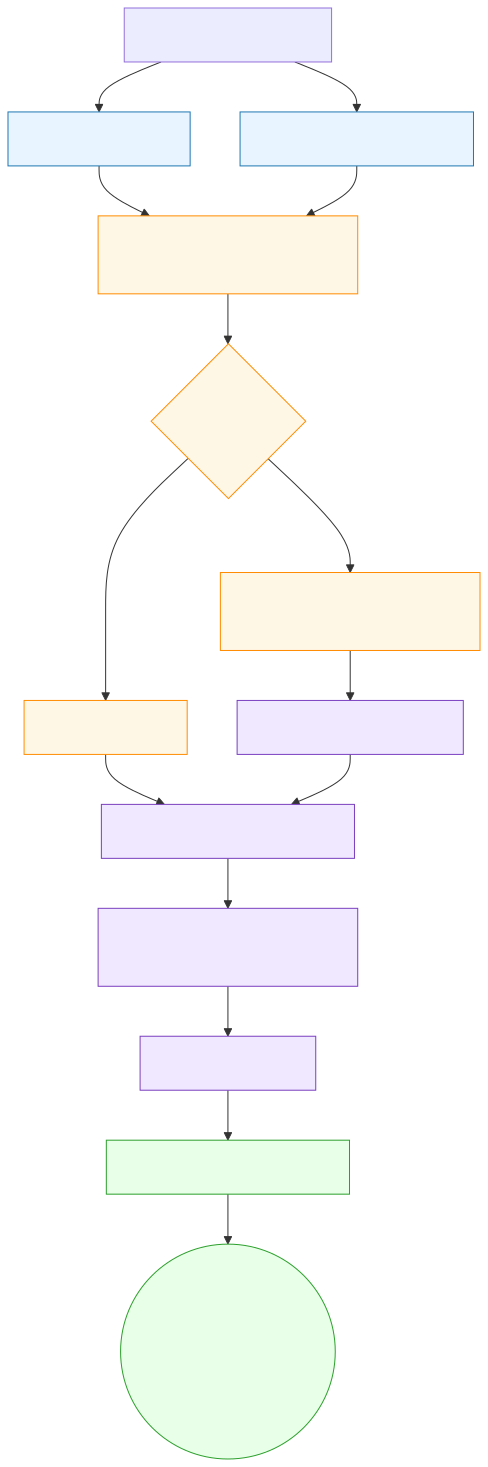
\includegraphics{src/images/diagrams/mobile_flow.pdf}
\end{adjustbox}
\caption{Mobile-side pipeline.}
\label{fig:mobile_pipeline}
\end{figure}

\section{Physical Limits}
\label{sec:physics}

Two physical reasons limit the ray-trace range to 30\,km. Earth curvature hides ridges beyond this distance. Atmospheric visibility also degrades --- contrast drops to about 10\% at 30\,km in clear mountain air. Full derivations are in Appendix~\ref{app:derivations}.

\begin{figure}[H]
\centering
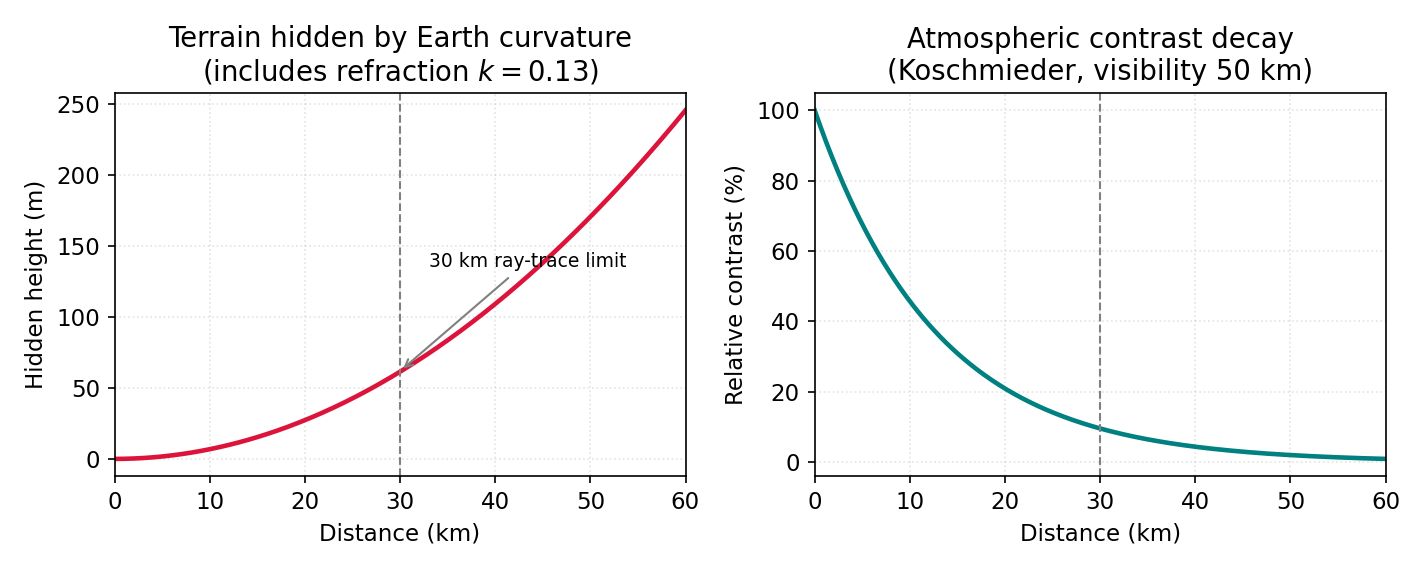
\includegraphics[width=0.82\textwidth]{src/images/figures/fig_physics_limits.png}
\caption{Curvature and contrast limits.}
\label{fig:physics_limits}
\end{figure}
